\documentclass[10pt,twoside,twocolumn]{article}

\usepackage{project}
\usepackage{graphicx}

\newcommand{\projecttitle}{Data Driven Improvements to RRT}
\newcommand{\authors}{Filipe Milit\~{a}o, Karl Naden,  Bernardo Toninho}
\newcommand{\projectdate}{\today}

\begin{document}

\maketitle

\section{Introduction} 
The RRT algorithm represents an extreme in the design space of planning algorithms.  
It forsakes optimality and explores the space through randomness and a small bias towards goals.  This is in marked contrast to other planning strategies such as visibility graphs or voronoi diagrams which carefully analyze and partition the space to find paths.  
This difference makes RRT very efficient even in higher dimensional spaces because its computational overhead is small in comparison to other algorithms which attempt to precisely characterize the world.  However, this also means that RRT does not take advantage of information that it learns about the world while exploring.

The central idea of our project is to introduce learning of the environment into the RRT algorithm for online use in the search and also for re-planning purposes.  We focus our efforts on the extension length for two reasons.  First, the RRT algorithm gets information about good and bad extension lengths from given points when it tests to see if a given extension fails.  Second, the optimal extension length varies based on the obstacles surrounding a given point.  The goal of this project is to extend the RRT planning and the ERRT re-planning algorithm to store and use information learned about good extension lengths while searching the space.  Our hope is that we can realize significant improvements in how fast and often RRT-based planning finds the goal, without sacrificing its key principles.

Our main goal is to explore a set of variations in the standard RRT (and ERRT) algorithms to try and offer a better algorithm for these heterogeneous worlds both in planning and re-planning scenarios.

Some other papers describing extensions to the RRT algorithm which include \cite{Lavalle98rapidly-exploringrandom},\cite{Lindemann04incrementallyreducing},\cite{Jaillet05adaptivetuning}, and \cite{moplan2009}.


\section{RRT Algorithms}

A Rapidly-exploring Random Tree (RRT) algorithm is a random algorithm designed for efficient search in
continuous spaces. The algorithm finds a path from a start point $S$ to a goal $G$ in a given search space 
by generating a random tree in the space. The tree will have $S$ as its root and is computed by randomly
choosing points in the world, finding the tree node $N$ closest to the random point and extending the tree by
creating a new node $N'$ connected to $N$, in the direction of the random point (as long as the extension does not
intersect any obstacles in the world). 

An immediate optimization to the algorithm in terms of path planning, called RRT-GoalBias, consists of adding a probability
parameter $p$, which causes the algorithm to choose to extend the tree towards the goal with probability $p$,
and extend towards a random point with probability $1-p$. 

The main advantages of using a RRT algorithm are that it does not require a discretization of the space and the high
efficiency in terms of time and space usage. Furthermore, it turns out that such a biased random exploration of the space
does indeed prove to be successful in finding paths, even in the presence of a large number of obstacles. Such positive
results have resulted in the usage of RRT for robot motion planning and re-planning (in the latter setting, information
about previous paths is also used to bias the search).

\subsection{Context Sensitivity}
Consider now a realistic scenario where the space in which we desire to plan has a high number of obstacles, possibly 
non-uniformly distributed throughout the world.
Such a world will have regions which will be fairly open, in which should be easy to find a path, and regions which will
be more cluttered and therefore harder to navigate through. The way RRT is used to find paths in such worlds, simply relies
on lowering the probability $p$ and the extension length. The first aims to avoid being stuck in the obstructed regions of the world,
while the latter aims to allow for extensions to succeed in these regions. Unfortunately, lowering these parameters naturally
decreases overall performance, since the algorithm extends less often towards the goal, and requires more extensions 
(and therefore more computation) to actually reach it, even in regions of the space where such a conservative approach may not be required.

Our observation is that RRT does not take advantage of the information it collects about the world, and therefore always employs a
rigid exploration tactic that needs to be globally conservative to succeed in the scenario above. However, it should be possible to use
the information collected throughout the exploration to adapt the tree generation procedure in such a way that the tree will cover
the less obstructed regions of space faster (in terms of computation time and number of nodes), all the while maintaining the ability
 to navigate through the more obstructed areas.
%
We address this issue by allowing the extension lengths between nodes to change over the course of the 
tree generation in such a way that the extension length becomes higher in open areas and lower in cluttered ones. Our basic framework
is as follows: we associate with each node in the tree an extension factor, which is used to determine the extension length that is to be
applied to all extensions from the node. Whenever an extension from a node fails, we decrease it's extension factor. 
When an extension succeeds, we increase the node's extension factor, generate the new node which will inherit the extension factor of its parent.

The idea is that we should always try to eagerly maximize the extension length, in order to cover space as fast as possible, therefore
as long as extensions succeed (and therefore the algorithm does not run into obstacles) it keeps increasing the extension length accordingly.
When the algorithm cannot extend from a node, it means that an obstacle exists in the proximity of that node and therefore the extension
length should decrease accordingly, to potentially increase the success of navigating through.

\subsubsection{VLRRT}

Variable Length RRT (VLRRT) is an algorithm that follows immediately in our framework. With each node of the tree,
we associate a value $\epsilon$ which is used as a multiplicative factor to the base extension length. For the root of the
tree, the value of $\epsilon$ starts off as $1$. As in standard RRT-GoalBias, the algorithm is parametrized with a probability of
extending towards the goal. The main difference lies in the treatment of the actual extensions. Whenever an extension from a given
node succeeds, we increase its $\epsilon$ value and generate the new node with the new $\epsilon$ value of its parent, in order to
propagate the extension information throughout the tree. Whenever an extension fails, we decrease the $\epsilon$ value of the node.

A natural question arises in this scenario, which is how to vary the $\epsilon$ value in the presence of successful and unsuccessful 
extensions. Therefore, we opted to parametrize the algorithm with three possible schemes with which to increase and/or decrease $\epsilon$:
a \emph{linear} scheme, in which $\epsilon$ increases/decreases a fixed amount; a \emph{multiplicative} scheme, in which $\epsilon$ is multiplied or divided by a fixed amount, and a \emph{restart} scheme, in which $\epsilon$ is restarted to its initial value of $1$.

\subsubsection{DVLRRT}
An immediate observation regarding VLRRT is that a successful or unsuccessful extension provides us information of the
presence or absence of obstacles in a particular direction, but not in all directions (which is the generalization that VLRRT employs). 
While such an over-generalization may indeed provide good results (which indeed turns out to be the case), it is clear that there
will be scenarios where $\epsilon$ will increase/decrease when perhaps it didn't need to. To take the extension idea one step
further, we developed Directional VLRRT (DVLRRT).

The idea behind DVLRRT is to account directionality into VLRRT's $\epsilon$ value modifications, in order to overcome the potential
downsides of the generalization employed in VLRRT. In each tree node, we store a \emph{directional $\epsilon$ map}. This 
structure maps a particular direction with an epsilon value, which enables us to take into account directions when updating $\epsilon$
and computing extension lengths.

Whenever we attempt to extend from a node in a given direction $d$, we check if a mapping with that particular direction exists in the directional map.
If so, we use the epsilon value stored in the map to compute the extension length and update it on failure/success as in VLRRT. If the mapping does not yet exist, we compute the $\epsilon$ value for the given direction by taking into account the directional information in the map: we look up directions similar to $d$ up to a certain angular distance, clockwise and counter-clockwise, and weight the information by proximity to $d$. We update the directional map with the $\epsilon$ value for $d$ on extension success/failure accordingly.

With this new strategy, we inform our extension length variation even further, by taking into account extension success and failure in directions that are similar to ones we have observed before in a node.


\section{Evaluating the algorithms}

To evaluate the performance of our algorithms, we implemented a simulation suite (with visualization) that allows
us to compare DVLRRT, VLRRT and RRT-GoalBias. The suite is also prepared for re-planning simulation, by simulating
random changes in worlds in successive iterations.

Our testing suite executes the specified algorithms (with a given time limit for each execution) in a number of previously
generated worlds and records relevant statistics such as time spent to find the goal, path length, world coverage, etc.

The metrics we used to compare DVLRRT, VLRRT and RRT-GoalBias for this report are success rate (in terms of finding the goal) and running
time. For DVLRRT and VLRRT, we also analyzed how the several $\epsilon$ modification schemes affect overall performance.

\section{Preliminary Results}

We executed each algorithm 10000 times, in several representative worlds, with a time limit of 50 milliseconds: 
a maze-like world \emph{maze} (similar to the one in
\cite{Bruce02real-timerandomized}), a largely unobstructed world with
a particularly obstructed region 
in the path to the goal \emph{obstructed} and a more highly cluttered world \emph{cluttered}.

We can observe that in all the test worlds, our algorithms perform
generally better (or as good) than RRT-GoalBias,
achieving higher average success rates and lower average execution
times, noting that in worlds where RRT-GoalBias already performs
very well, the gains achieved by our algorithms are naturally smaller.

However, and not unexpectedly, the performance increase of our algorithms does not occur for all
$\epsilon$ modification schemes.
Our intuition was that we wanted to ``speed through'' what we consider to be unobstructed regions, but decrease our
``speed'' as fast as possible when we find an obstructed region, so we can effectively navigate through it. As it turns
out, our intuition is indeed correct, seeing as the modification schemes that perform the best are those that
increase $\epsilon$ faster but decrease $\epsilon$ even faster, in both VLRRT and DVLRRT. Particularly, the best
results were obtained when the increase rate was the highest (multplicative scheme) and the decrease rate was the 
highest as well (restarting scheme). For the sake of readability, we
omit the results regarding other modification schemes, noting that, in
general, choosing a ``slow'' decrease rate produces overall bad
results.

Analyzing the actual values (Fig.~\ref{fig:worlds}), we can see that in the \emph{obstructed}
world, RRT-GoalBias already performs very well, therefore our gains
are less considerable. In fact, we gain a marginal overhead in terms
of time due to extra computation. In the \emph{maze} world,
RRT-GoalBias performs a bit worse, since the world is generally more
complex. In this world, our algorithms start to shine. Not only do
they find they goal almost $100\%$ of the runs, they actually find the
goal faster. This shows that our algorithms are indeed able to
navigate such worlds faster and more successfully, given that they can
adapt themselves to the world in question.
Finally, in the \emph{cluttered} world, RRT-GoalBias does not fair
well at all, given the high degree of heterogeneity in the world. Our
algorithms however (not unexpectedly), 
manage to not only find paths to the goal more frequently
(approx. twice as better), but also do so faster. 
Overall, we can conclude that our algorithms obtain an increase
of success rate (in terms of finding the goal) of approximately
$16\%$ and a decrease in running time of approximately $15\%$,
depending on the type of world we consider.

To conclude, our preliminary results further increase our confidence that our approach can indeed produce effective gains in
planning and that exploiting the gathered information for re-planning purposes should increase the performance gains
even further.

\begin{figure}[t]
\begin{center}
\footnotesize{
\begin{tabular}{|cccc|}
\hline
Algorithm & World & Avg. & Avg.\\
& & Success & Time (ms.)\\
\hline
RRT-GoalBias & obstr. & 95\% & 11.94\\
VLRRT (M2/R) & obstr. & 96\% & 13.48\\
VLRRT (M4/R) & obstr. & 95\% & 13.32\\
DVLRRT (M2/R1) & obstr. & 96\% & 13.65\\
DVLRRT (M3/R1) & obstr. & 96\% & 13.41\\
DVLRRT (M4/R1) & obstr. & 96\% & 13.38\\
VLRRT (M3/R1) & obstr. & 95\% & 13.61\\ 
\hline
RRT-GoalBias & maze & 91\% & 17.26\\
VLRRT (M2/R) & maze & 99\% & 10.59\\
VLRRT (M4/R) & maze & 99\% & 10.60\\
DVLRRT (M2/R1) & maze & 99\% & 10.50\\
DVLRRT (M3/R1) & maze & 99\% & 10.69\\
DVLRRT (M4/R1) & maze & 99\% & 10.74\\
VLRRT (M3/R1) & maze & 99\% & 10.69\\ 
\hline
RRT-GoalBias & clutt. & 33\% & 39.26\\
VLRRT (M2/R) & clutt. & 60\% & 34.00\\
VLRRT (M4/R) & clutt. & 59\% & 33.61\\
DVLRRT (M2/R1) & clutt. & 60\% & 33.86\\
DVLRRT (M3/R1) & clutt. & 60\% & 33.73\\
DVLRRT (M4/R1) & clutt. & 60\% & 33.89\\
VLRRT (M3/R1) & clutt. & 60\% & 33.90\\ 
\hline
\end{tabular}}
\end{center}
\caption{Success Rates and Exec. Times}\label{fig:worlds}
\end{figure}
\begin{figure}[t]
\begin{center}
\footnotesize{
\begin{tabular}{|ccc|}
\hline
Algorithm & Avg. Succ. Rate & Avg. Time\\
\hline
VLRRT (M2/R) & 17\% & -15\%\\
VLRRT (M4/R) & 16\% & -16\%\\
DVLRRT (M2/R1) & 17\% & -15\%\\
DVLRRT (M3/R1) & 16\% & -16\%\\
DVLRRT (M4/R1) & 17\% & -15\%\\
VLRRT (M3/R1) & 16\% & -15\%\\ 
\hline
\end{tabular}}
\end{center}
\caption{Overall Gains versus RRT}
\end{figure}

\section{Progress and Future Steps}

We have successfully implemented and evaluated two strategies that improve RRT-GoalBias by
taking into account information about the world during planning. We will now
direct our efforts into using the collected information to further improve performance
in re-planning scenarios (in comparison to ERRT). 

Our claim is that if the information we collect
about the world does indeed produce good results, then we should be able to incorporate that
information in subsequent executions (i.e re-planning) by extrapolating the unobstructed regions of
the world from the $\epsilon$ values of the previous executions. A possible way to do this is
to generate the regions using a K-Nearest Neighbors algorithm \cite{citeulike:995135}. Under the reasonable assumption
that the world doesn't change too much between executions, we can use the region information to
\emph{a priori} inform the $\epsilon$ values of points that fall
within said regions.

\section{Re-planning}

asd

\section{Conclusions}

asd

\bibliography{AIbib}{}
\bibliographystyle{alpha}

\appendix 
\section{World Images}
\begin{figure}[h]
\begin{center}
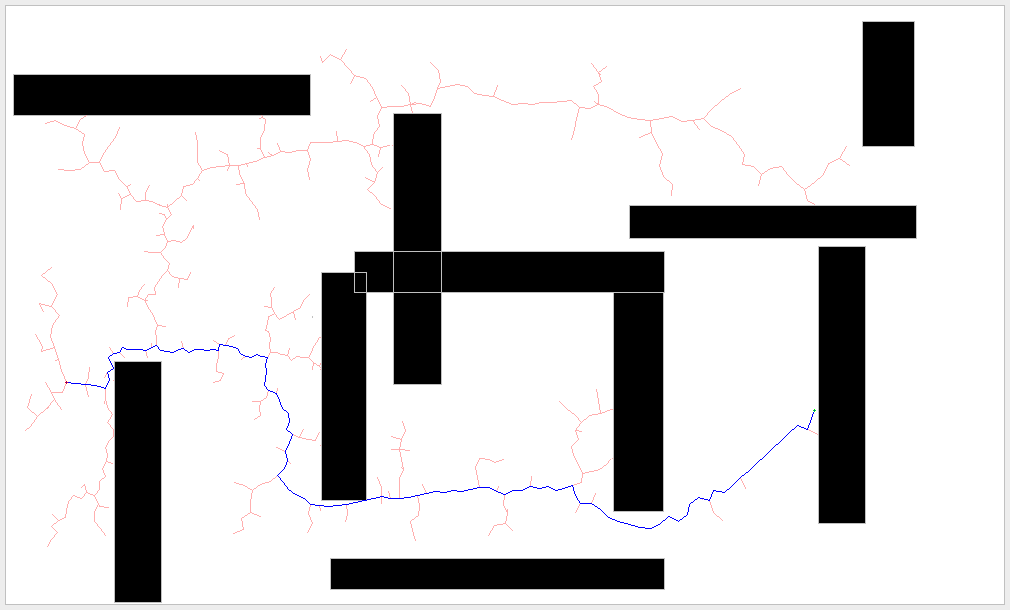
\includegraphics[scale=0.20]{paper_world.png}
\end{center}
\caption{Maze World}
\end{figure}
\begin{figure}[h]
\begin{center}
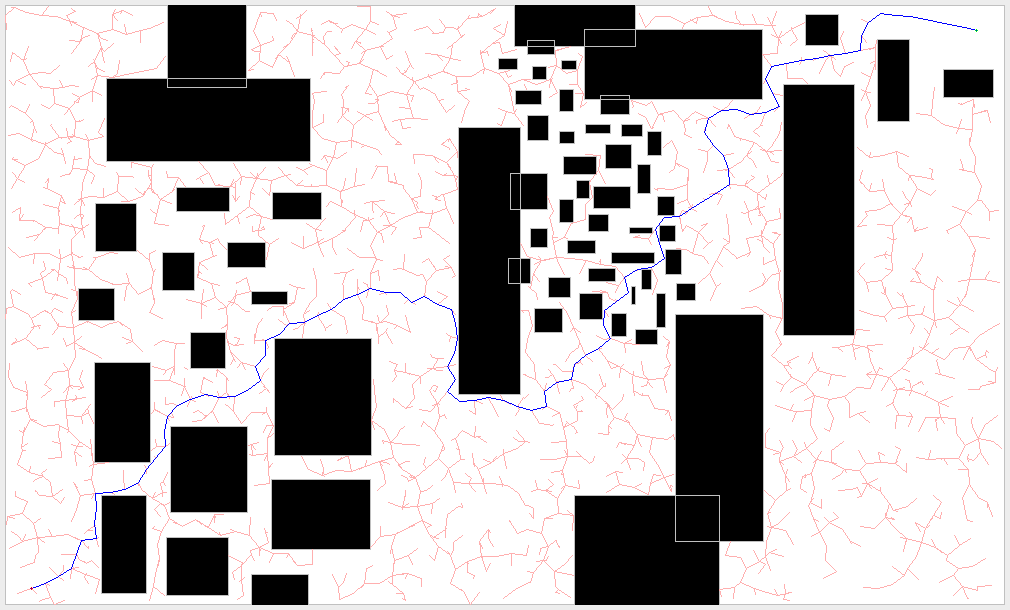
\includegraphics[scale=0.2]{cluttered_world.png}
\end{center}
\caption{Cluttered World}
\end{figure}
\begin{figure}[h]
\begin{center}
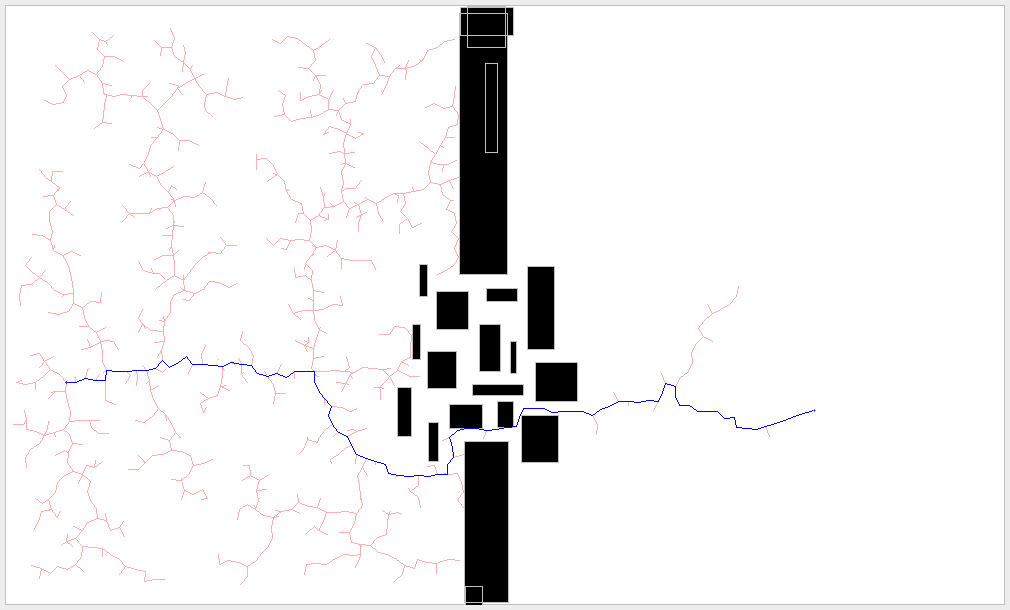
\includegraphics[scale=0.2]{prop_world.png}
\end{center}
\caption{Obstructed World}
\end{figure}

\section{Results}

\begin{figure}[h]
\begin{center}
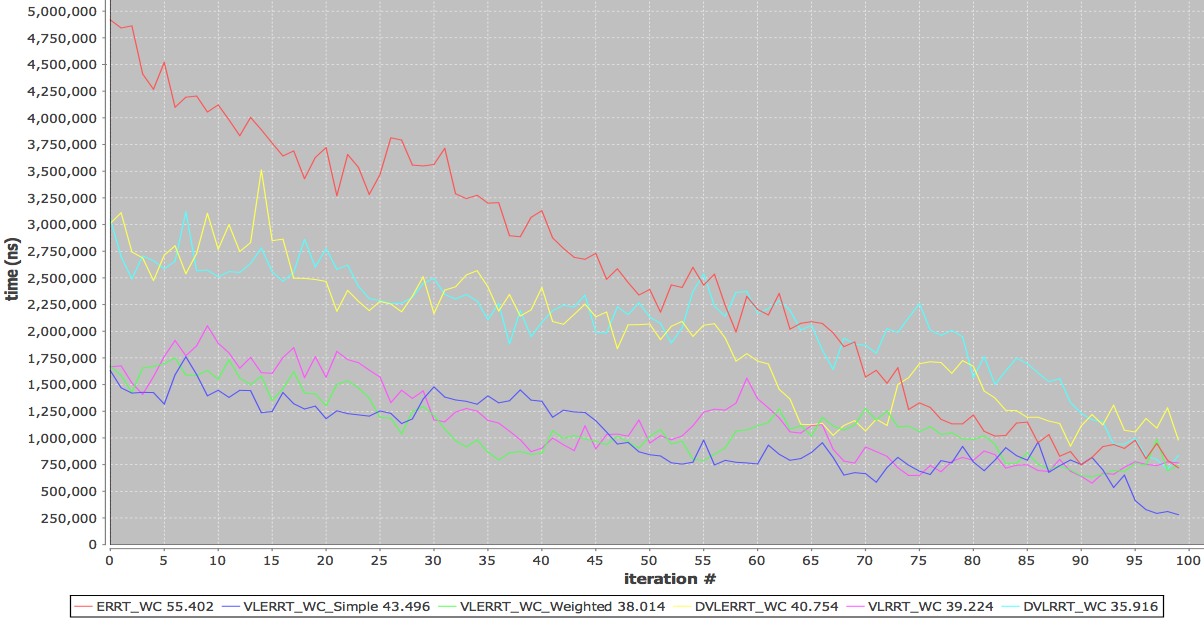
\includegraphics[scale=0.2]{maze_wc.png}
\end{center}
\caption{Maze re-planning.}
\end{figure}


\begin{figure}[h]
\begin{center}
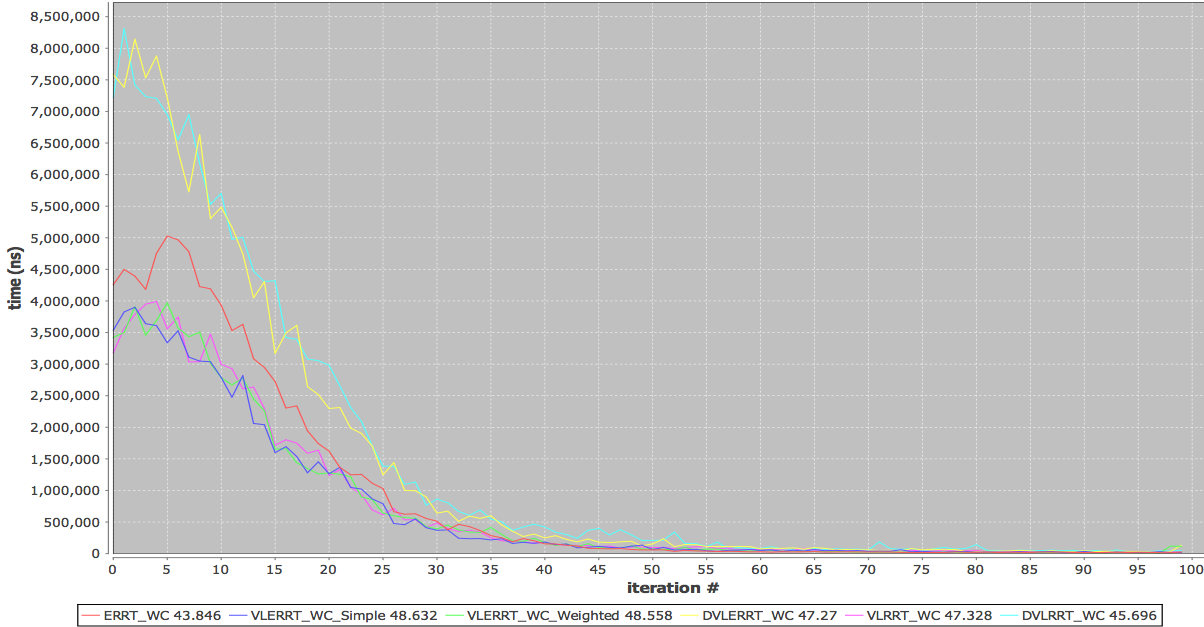
\includegraphics[scale=0.2]{obstructed_wc.png}
\end{center}
\caption{Obstructed re-planning.}
\end{figure}


\begin{figure}[h]
\begin{center}
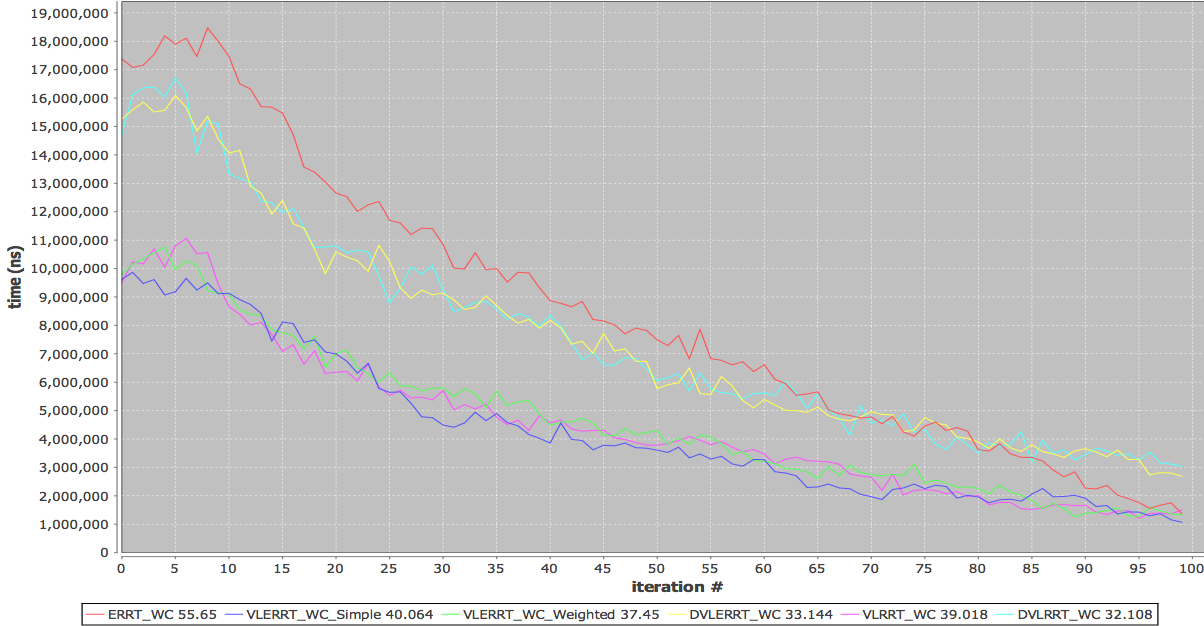
\includegraphics[scale=0.2]{cluttered_wc.png}
\end{center}
\caption{Cluttered re-planning.}
\end{figure}

\end{document}

